\section{Introduction}
\begin{itemize}
    \item Port numbers, TCP, and UDP.
\end{itemize}


%----------------------------------------------------------------------------------------
\section{Layer 4 - The transport layer}
\begin{itemize}
    \item The transparent layer provides transparent transfer of data between hosts and is responsable for end-to-end error recovery and flow control.
        \begin{itemize}
            \item Error recovery and flow control are not mandatory, some layer 4's will and others will not.
        \end{itemize}
    
    \item Flow control is the process of adjusting the flow of data from the ender to ensure that the receiving host can handle all of it.
        \begin{itemize}
            \item Example: If the sender is sending data at a faster rate than the reciever can handle then the flow control will have a mechanism that can go back to the sender to tell it to slow down.
        \end{itemize}
    
    \item Session multiplexing is the process by which a host is able to support multiple sessions simultaneously and manage individual traffic streams over a single link.
        \begin{figure}[H]
            \centering
            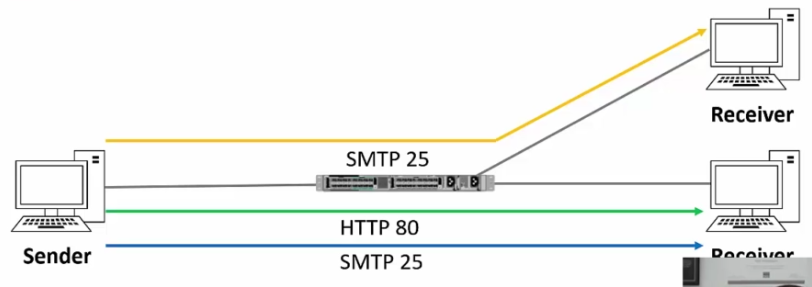
\includegraphics[width=0.4\textwidth]{./Figs/2022-01-04-22-08-33.png}
        % 	\caption{}
        \end{figure}
        \begin{itemize}
            \item Notice that the sender has three sessions, has a SMTP session running in port 25, http session in port 80 and SMTP in port 25. It is the job of LAYER 4 THE TRANSPORT LAYER to keep track and control of all the sessions on our host.
        \end{itemize}
\end{itemize}

\subsection{Port numbers}
\begin{itemize}
    \item The layer 4 destination port number is used to identify the upper layer protocol.
    \item For example, HTTP uses port 80, SMTP email uses port 25, etc.
    \item The sender also adds a source port number to the layer 4 header.
    \item The combination of source and destination port number can be used to track session.
    \item For example, when a receiver host receiver a packet, it knows to which application to use it by its port number. If it comes in port 25 we know its comming for email application.
\end{itemize}
\begin{figure}[H]
    \centering
    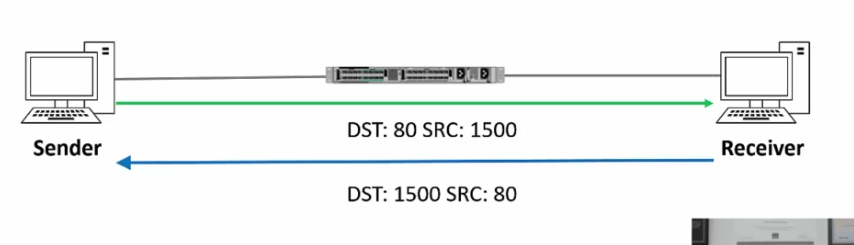
\includegraphics[width=0.4\textwidth]{./Figs/2022-01-04-22-16-27.png}
% 	\caption{}
\end{figure}
\begin{itemize}
    \item When the sender sends the traffic to the receiver it will specify the destination and source port number, in the above example we are using port 80 and 1500, if traffic is expected to be returned then the receiver will flip the destination and source port numbers so that the source is now 80 and the destination is 1500.
    \item This is how state 4 firewalls are able to keep track of connections. We can restrict traffic in both directions or just in one, for example a firewall can restrict traffic from the receiver to the sender unless the sender has initiated communication with the receiver first.
\end{itemize}

\subsection{TCP}
\begin{itemize}
    \item TCP:
        \begin{itemize}
            \item TCP is one of two most common protocols in layer 4. TCP (Transport Control Protocol) and UDP (the User Datagram Protocol) are the two most popular.
            \item TCP is connection oriented: once a connection is established, data can be sent bidirectionally over that connection.
            \item TCP is reliable: the receiving host sends acknowledgments back to the sender. Lost segments are resent. When a segment of data is lost the receiver will not send an acknowledgement to the sender and this will prompt the sender to resend the lost segment of data.
            \item TCP performs flow control (remember its like synchronization between the sender and receiver so that the flow of data is received at a speed that is managable for the receiver).
            \item TCP tends to have the opposite characteristics to UDP.
        \end{itemize}

    \item The TCP Three-way handshake
        \begin{itemize}
            \item The way that a TCP connection is set up is via the TCP three-way hand shake.
                \begin{figure}[H]
                    \centering
                    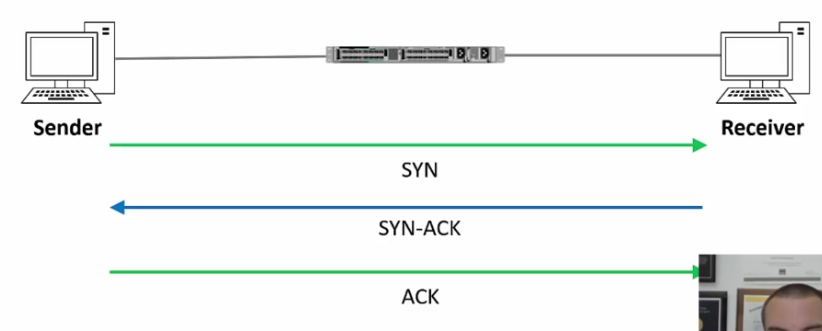
\includegraphics[width=0.4\textwidth]{./Figs/2022-01-04-22-28-51.png}
                % 	\caption{}
                \end{figure}
            \item The way the three-way hand shake occurs is that it first sends a SYN message, SYN is short for synchronization message, when the receiver gets the SYN message it returns a SYN-ACK -- which is shot for synchronization message acknowledgement -- allowing it to complete the connection and now the two hosts have the connection and they can send traffic to each other, this is the 'third' step, that now that the sender has received a SYN-ACK they have established a connection and can send each other stuff.
        \end{itemize}
    
    \item The TCP Header:
        \begin{itemize}
            \item \item *Reminder: TCP packet header has all of the following:
            \begin{figure}[H]
                \centering
                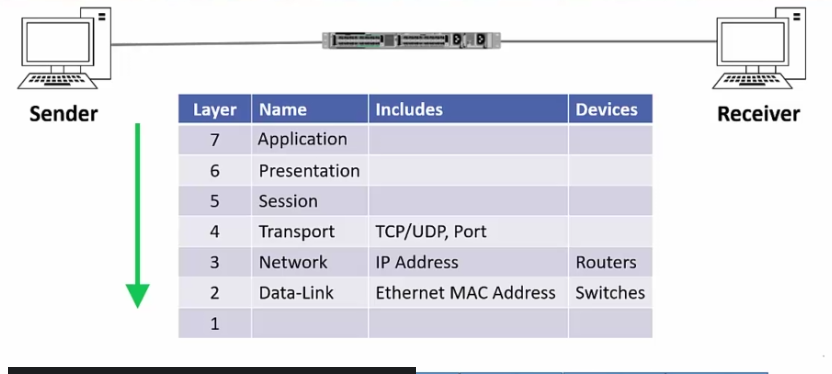
\includegraphics[width=0.4\textwidth]{./Figs/2022-01-04-22-33-06.png}
            % 	\caption{}
            \end{figure}
        
            \item Now a packet is assembled as follows:
                \begin{figure}[H]
                    \centering
                    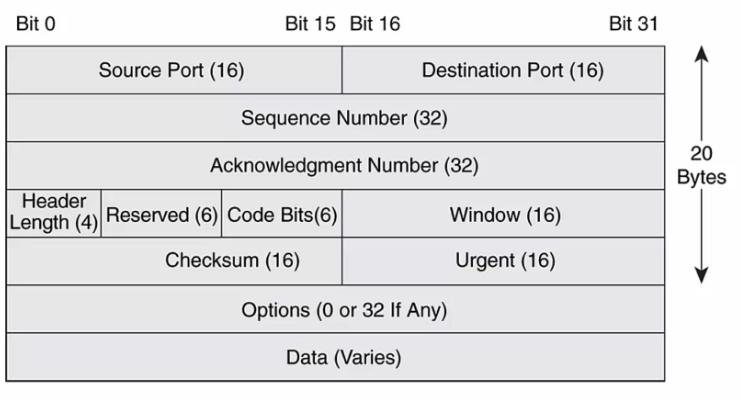
\includegraphics[width=0.4\textwidth]{./Figs/2022-01-04-22-34-15.png}
                % 	\caption{}
                \end{figure}
                \begin{itemize}
                    \item We have all the fields represented by bits on a long word that comprices the packet. The first 16 bits of the packet stores the source port, the next 16 the destination port, and so on. This is very similar to how an assembler instruction is assembled in a microprocessor.
                \end{itemize}
        \end{itemize}
\end{itemize}


\subsection{UDP}
\begin{itemize}
    \item UDP:
        \begin{itemize}
            \item The UDP is User Datagram Protocol, it sends traffic best effort.
            \item UDP is not connection oriented. There is no handshake connection setup between the hosts.
            \item UDP does not carry out sequencing to ensure segments are processed in the correct order nor checks if they are missing.
            \item UDP is not reliable: the receiving host does not send acknowledgements back to the sender.
            \item UDP does not perform flow control.
            \item If error detection and recovery is required it is up to the upper layers to provide it, it is NOT provided by UDP.
        \end{itemize}
    
    \item The UDP Header:
        \begin{itemize}
            \item In the UDP header we have much less fields compared to the TCP. Observe:
                \begin{figure}[H]
                    \centering
                    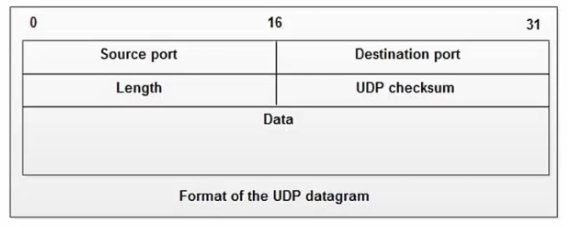
\includegraphics[width=0.4\textwidth]{./Figs/2022-01-04-22-43-15.png}
                % 	\caption{}
                \end{figure}
            
            \item We only have the destination and source ports, length, UDP checksum, and the data.
            \item This is both and advantage and a liability. With UDP you get much less overhead for example.
        \end{itemize}
\end{itemize}

\subsection{UDP vs TCP}
\begin{itemize}
    \item TCP and UDP have different use cases.
    \item Application developers will typically choose to use TCP for traffic which requires reliability.
    \item For example: real-time applications such as voice and video can't afford the extra overhead of TCP so they use UDP. If we were to use TCP on real time applications we would probably get large amounts of lagging and latency, because of the extra overhead, this would affect the quality and make it imposable to interact in real time, in such a case an unreliable connection with less header overhead is much appreciated.
    \item Some applications can use both TCP and UDP.
    \item TCP is the most commonly used protocol.
\end{itemize}

\subsection{Common applications and their destination ports}
\begin{center}
    \begin{tabular}{ |p{5cm}|p{5cm}|p{5cm}| }
        \hline
            TCP & UDP & TCP and UDP \\
        \hline
            {
                \begin{itemize}
                    \item FTP (PORT 21)
                    \item SSH (PORT 22)
                    \item TELNET (PORT 23)
                    \item HTTP (PORT 80)
                    \item HTTPS (PORT 443)
                \end{itemize}
            }
             &
            {
                \begin{itemize}
                    \item TFTP (PORT 69)
                    \item SNMP (PORT 161)
                \end{itemize} 
            }
            & 
            {
                \begin{itemize}
                    \item DNS (PORT 53)
                \end{itemize} 
            } 
            \\
        \hline
    \end{tabular}
\end{center}

